
\documentclass[border=10pt]{standalone}
\usepackage{tikz}
\begin{document}
    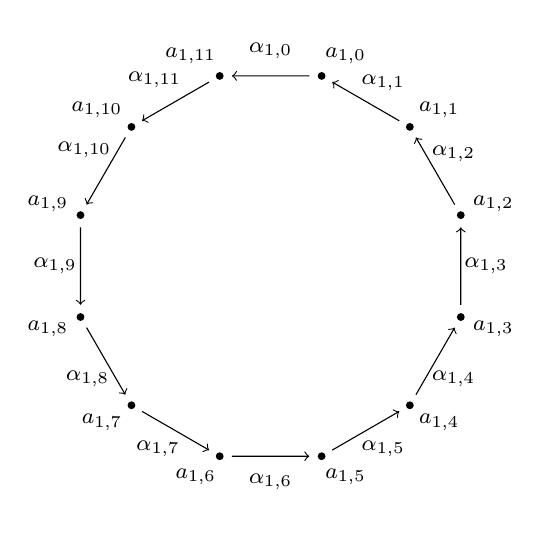
\begin{tikzpicture}[rotate=120,]% rotate=120
    \foreach \i [
      count=\j from -1, % trick to start from -1
      evaluate=\i as \invi using int(11-\i),
      evaluate=\j as \invj using int(11-\j),
    ] in {0,...,11} {
        \node[
          fill, circle, 
          inner sep=1pt, outer sep=3pt,
          label={
            [inner sep=0pt, minimum width=.5em,]
            {360/12*(\i-1/2)+120}:{\footnotesize $a_{1,\invi}$}
          }
        ] (a\i) at ({360/12*(\i-1/2)}:2.5) {};
        \ifnum\i=0\else
            \draw[<-] (a\i) -- node[inner sep=0pt, circle, label={
                [circle, inner sep=0pt]{360/12*(\i-1)+120}:{\footnotesize$\alpha_{1,\invj}$}
            }] {} (a\j);
        \fi
    }
    \draw[<-] (a0) -- node[
      inner sep=0pt, circle,
      label={
        [circle, inner sep=0pt, swap]
        {-360/12+120}:{\footnotesize$\alpha_{1,0}$}
    }] {} (a11);
    \end{tikzpicture}
\end{document}